\section{Results}

Across all the censuses and traps/subplots, the data contained 666 species of trees, 26 species of small-mammals and 58 families of beetles. Output from the PCAs performed on each taxa separately but including all subplots/traps and census indicated that the first 3 components explained 28.89\%, 5.65\%, 4.44\% (cumulative 38.98\%) for trees, 26.44\%, 24.03\%, 11.34\% (cumulative 61.81\%) for mammals and 88.33\%, 7.59\%, 1.87\% (cumulative 97.79\%) for beetles.


\subsection{Comparison of Hypervolumes}

Hypervolumes were constructed for all plots and census and each census step within plots was compared. Figure \ref{fig:1} shows an example of a stable plot with little change in hypervolume shape leading to high levels of overlap and a comparatively unstable plot where significant changes in shape and size of the hypervolume lead to smaller measure of overlap and greater distance between centroids.

\begin{figure}[H]
	\centering
	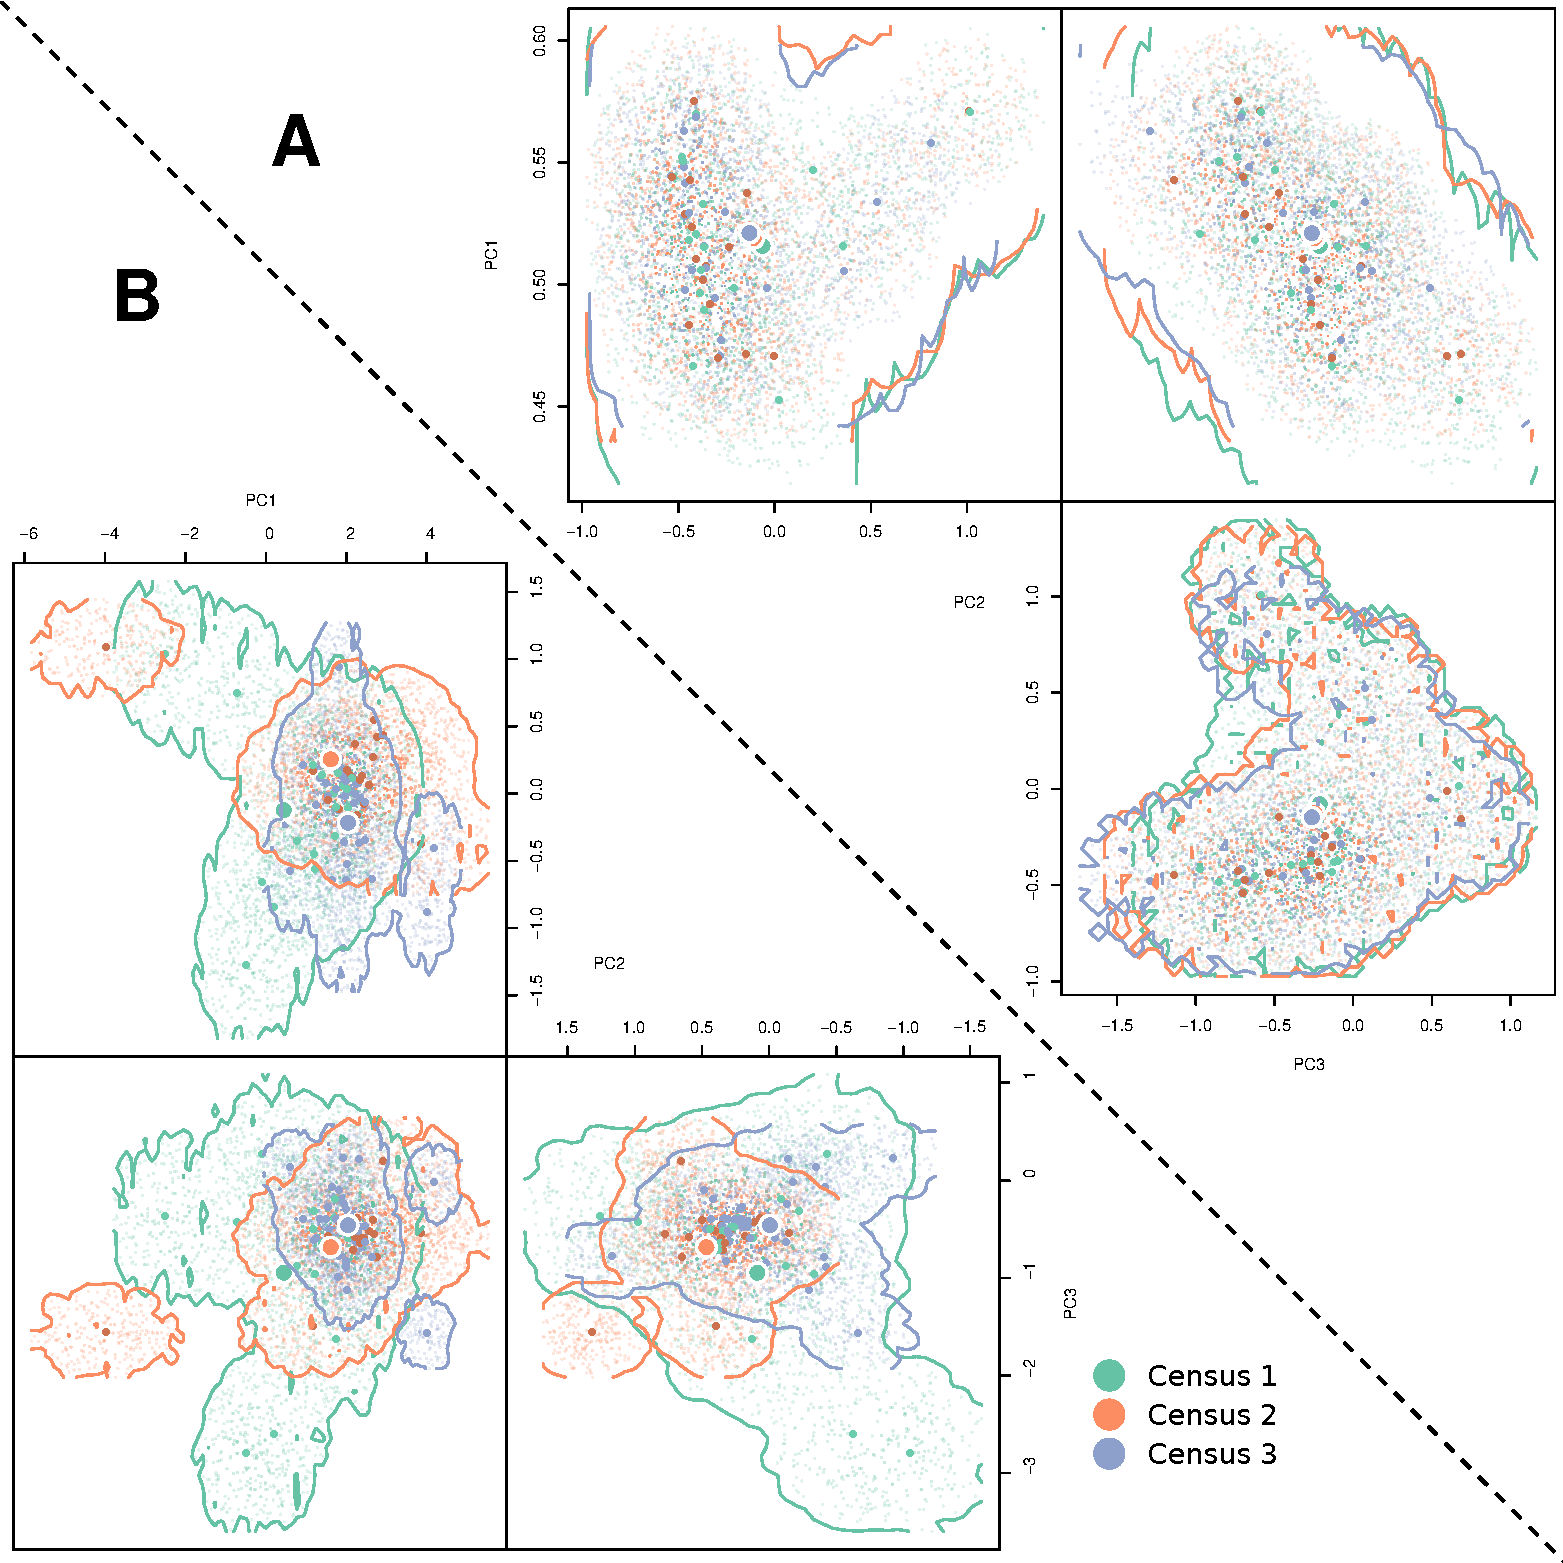
\includegraphics[width=\textwidth]{figures/figure1.pdf}
	\caption{(A) Hypervolumes constructed from tree community data at the Belian plot, an example of a plot with high levels of hypervolume overlap (mean = 0.802). (B) Hypervolume constructed from beetles community data at plot D, an example of comparativley low hypervolume overlap (mean = 0.243)}
	\label{fig:1}
\end{figure}	


\subsection{Effect of Taxa and Aboveground Biomass}

A one-way ANOVA found a significant difference in hypervolume overlap between taxa (F(2, 60) = 151.1, p < 0.001), with a post-hoc Tukey HSD finding that trees have significantly higher levels of overlap when compared with mammals or beetles (p < 0.001) (figure \ref{fig:2} A \& B), while no difference was found between the other taxa. No significant effect of AGB was found to exist with the level of hypervolume overlap in any of the taxa, results summarised in Table \ref{tab:hv-ovlp}.

\begin{figure}[H]
	\centering
	\includegraphics[width=\textwidth]{figures/figure2.pdf}
	\caption{(A) Difference in hypervolume overlap between taxa. (B) Effect of AGB on hypervolume overlap. (C) Difference in temporal community stability between taxa. (B) Effect of AGB on temporal community stability.}
	\label{fig:2}
\end{figure}

\begin{table}[H]
	\singlespacing
	\caption{Summary of results from ANCOVA assessing the relationship of taxa and AGB to hypervolume overlap}
	\label{tab:hv-ovlp}
	\begin{tabular*}{\textwidth}{c @{\extracolsep{\fill}} @{}llllll@{}}
		\toprule
		& \textbf{Df} & \textbf{Sum Squares} & \textbf{Mean Square} & \textbf{F Value} & \textbf{p} \\ \midrule
		log(AGB)    & 1  & 0.049       & 0.0492      & 3.043   & 0.087   \\
		Taxa        & 2  & 5.026       & 2.5128      & 155.439 & < 0.001 \\
		Interaction & 2  & 0.066       & 0.0332      & 2.053   & 0.138   \\
		Residuals   & 57 & 0.921       & 0.0162      &         &         \\ \bottomrule
	\end{tabular*}
\end{table}


\subsection{Community Temporal Stability}

A similar pattern was found with this more traditional measure of stability, with trees having significantly higher levels of temporal stability than either of the other taxa (F(2, 27) = 46.79, p < 0.001). With this measure there was an effect of AGB on the stability in trees (figure \ref{fig:2}D) however again this did not exist for the other taxa results summarised in Table \ref{tab:stb-ovlp}.

\begin{table}[H]
	\singlespacing
	\caption{Summary of results from ANCOVA assessing the relationship of taxa and AGB to community temporal stability}
	\label{tab:stb-ovlp}
	\begin{tabular*}{\textwidth}{c @{\extracolsep{\fill}} @{}llllll@{}}
		\toprule
		& \textbf{Df} & \textbf{Sum Squares} & \textbf{Mean Square} & \textbf{F Value} & \textbf{p} \\ \midrule
		log(AGB)    & 1  & 6.31       & 6.306      & 13.063   & 0.001   \\
		Taxa        & 2  & 57.09       & 28.545      & 59.133 & < 0.001 \\
		Interaction & 2  & 4.45       & 2.223      & 4.605   & 0.0203   \\
		Residuals   & 24 & 11.59       & 0.483      &         &         \\ \bottomrule
	\end{tabular*}
\end{table}

A significant Pearson's correlation was found between this new measure of stability 'Hypervolume Overlap' and the community temporal stability for each plot (r = 10.93, df = 28, p < 0.001) (figure \ref{fig:3}). However this relationship did not exist when looking at individual taxa in turn, with the exception of trees (r = 3.82, df = 7, p = 0.007).

\begin{figure}[H]	
	\centering
	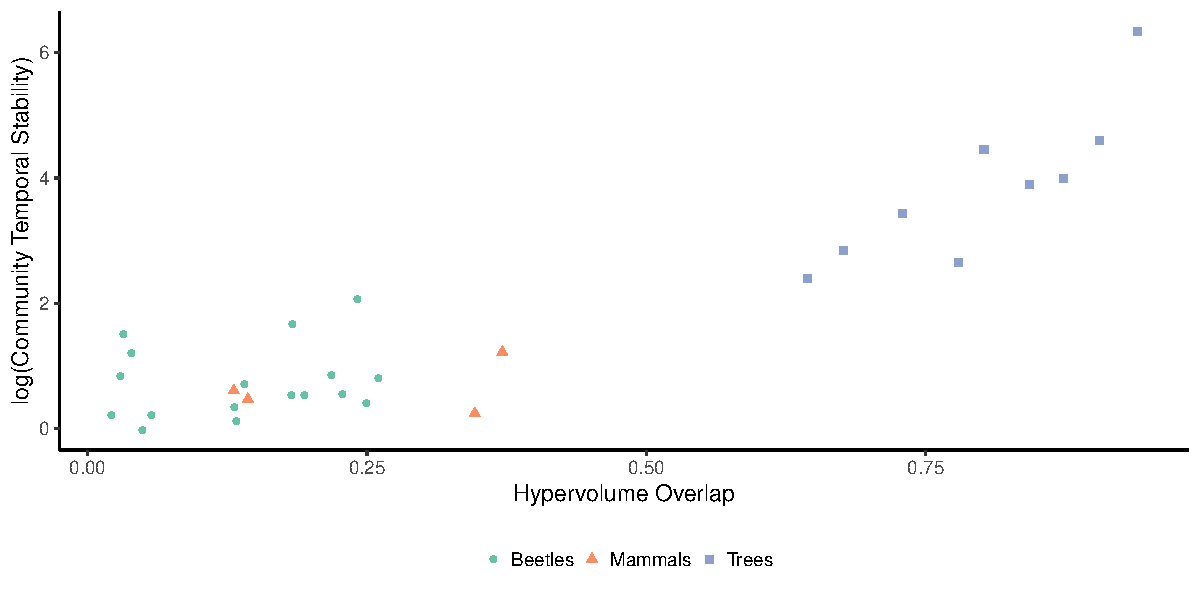
\includegraphics[width=\textwidth]{figures/figure3.pdf}
	\caption{The relationship between hypervolume overlap and temporal community stability. A significant Pearson's correlation was found overall (r = 10.93, df = 28, p < 0.001). However when split into separate taxa only trees had a significant correlation (r = 3.82, df = 7, p = 0.007)}
	\label{fig:3}
\end{figure}
